\documentclass{article}
\usepackage[utf8]{inputenc}

\title{Essay 4 - Ice Age Geography}
\author{Benny Chen}
\date{\today}

\usepackage{color}
\usepackage{amsthm}
\usepackage{amssymb} 
\usepackage{amsmath}
\usepackage{listings}
\usepackage{xcolor}
\usepackage{listings}
\usepackage{graphicx}
\usepackage[hidelinks]{hyperref}

\definecolor{codegreen}{rgb}{0,0.6,0}
\definecolor{codegray}{rgb}{0.5,0.5,0.5}
\definecolor{codepurple}{rgb}{0.58,0,0.82}
\definecolor{backcolour}{rgb}{0.95,0.95,0.92}

\lstdefinestyle{mystyle}{
    backgroundcolor=\color{backcolour},   
    commentstyle=\color{codegreen},
    keywordstyle=\color{magenta},
    numberstyle=\tiny\color{codegray},
    stringstyle=\color{codepurple},
    basicstyle=\ttfamily\footnotesize,
    breakatwhitespace=false,         
    breaklines=true,                 
    captionpos=b,                    
    keepspaces=true,                 
    numbers=left,                    
    numbersep=5pt,                  
    showspaces=false,                
    showstringspaces=false,
    showtabs=false,                  
    tabsize=2
}

\lstset{style=mystyle}

\begin{document}

\maketitle

In the video ``The Geography of the Ice Age'', the narrator talks about the geography of the world thousands of years ago. There were many land masses connected to each other then but not now. One of these connecting land masses was Russia to America, or Alaska. This land mass was called Beringia. There was also connections on in Asia. Japan was connected to the rest of Asia. This was due to the sea levels dropping and the land mass of Japan being exposed. Lastly, in Eurpoe, there was a land mass connecting the United Kingdom was connected to the rest of Europe. This was called Doggerland. This connected Britain, Ireland, and Scandinavia. This land mass was also exposed due to the sea levels dropping. 

\begin{center}
    \includegraphics[width=0.5\textwidth]{land1.png}
\end{center}

\begin{center}
    \includegraphics[width=0.5\textwidth]{land2.png}
\end{center}

\begin{center}
    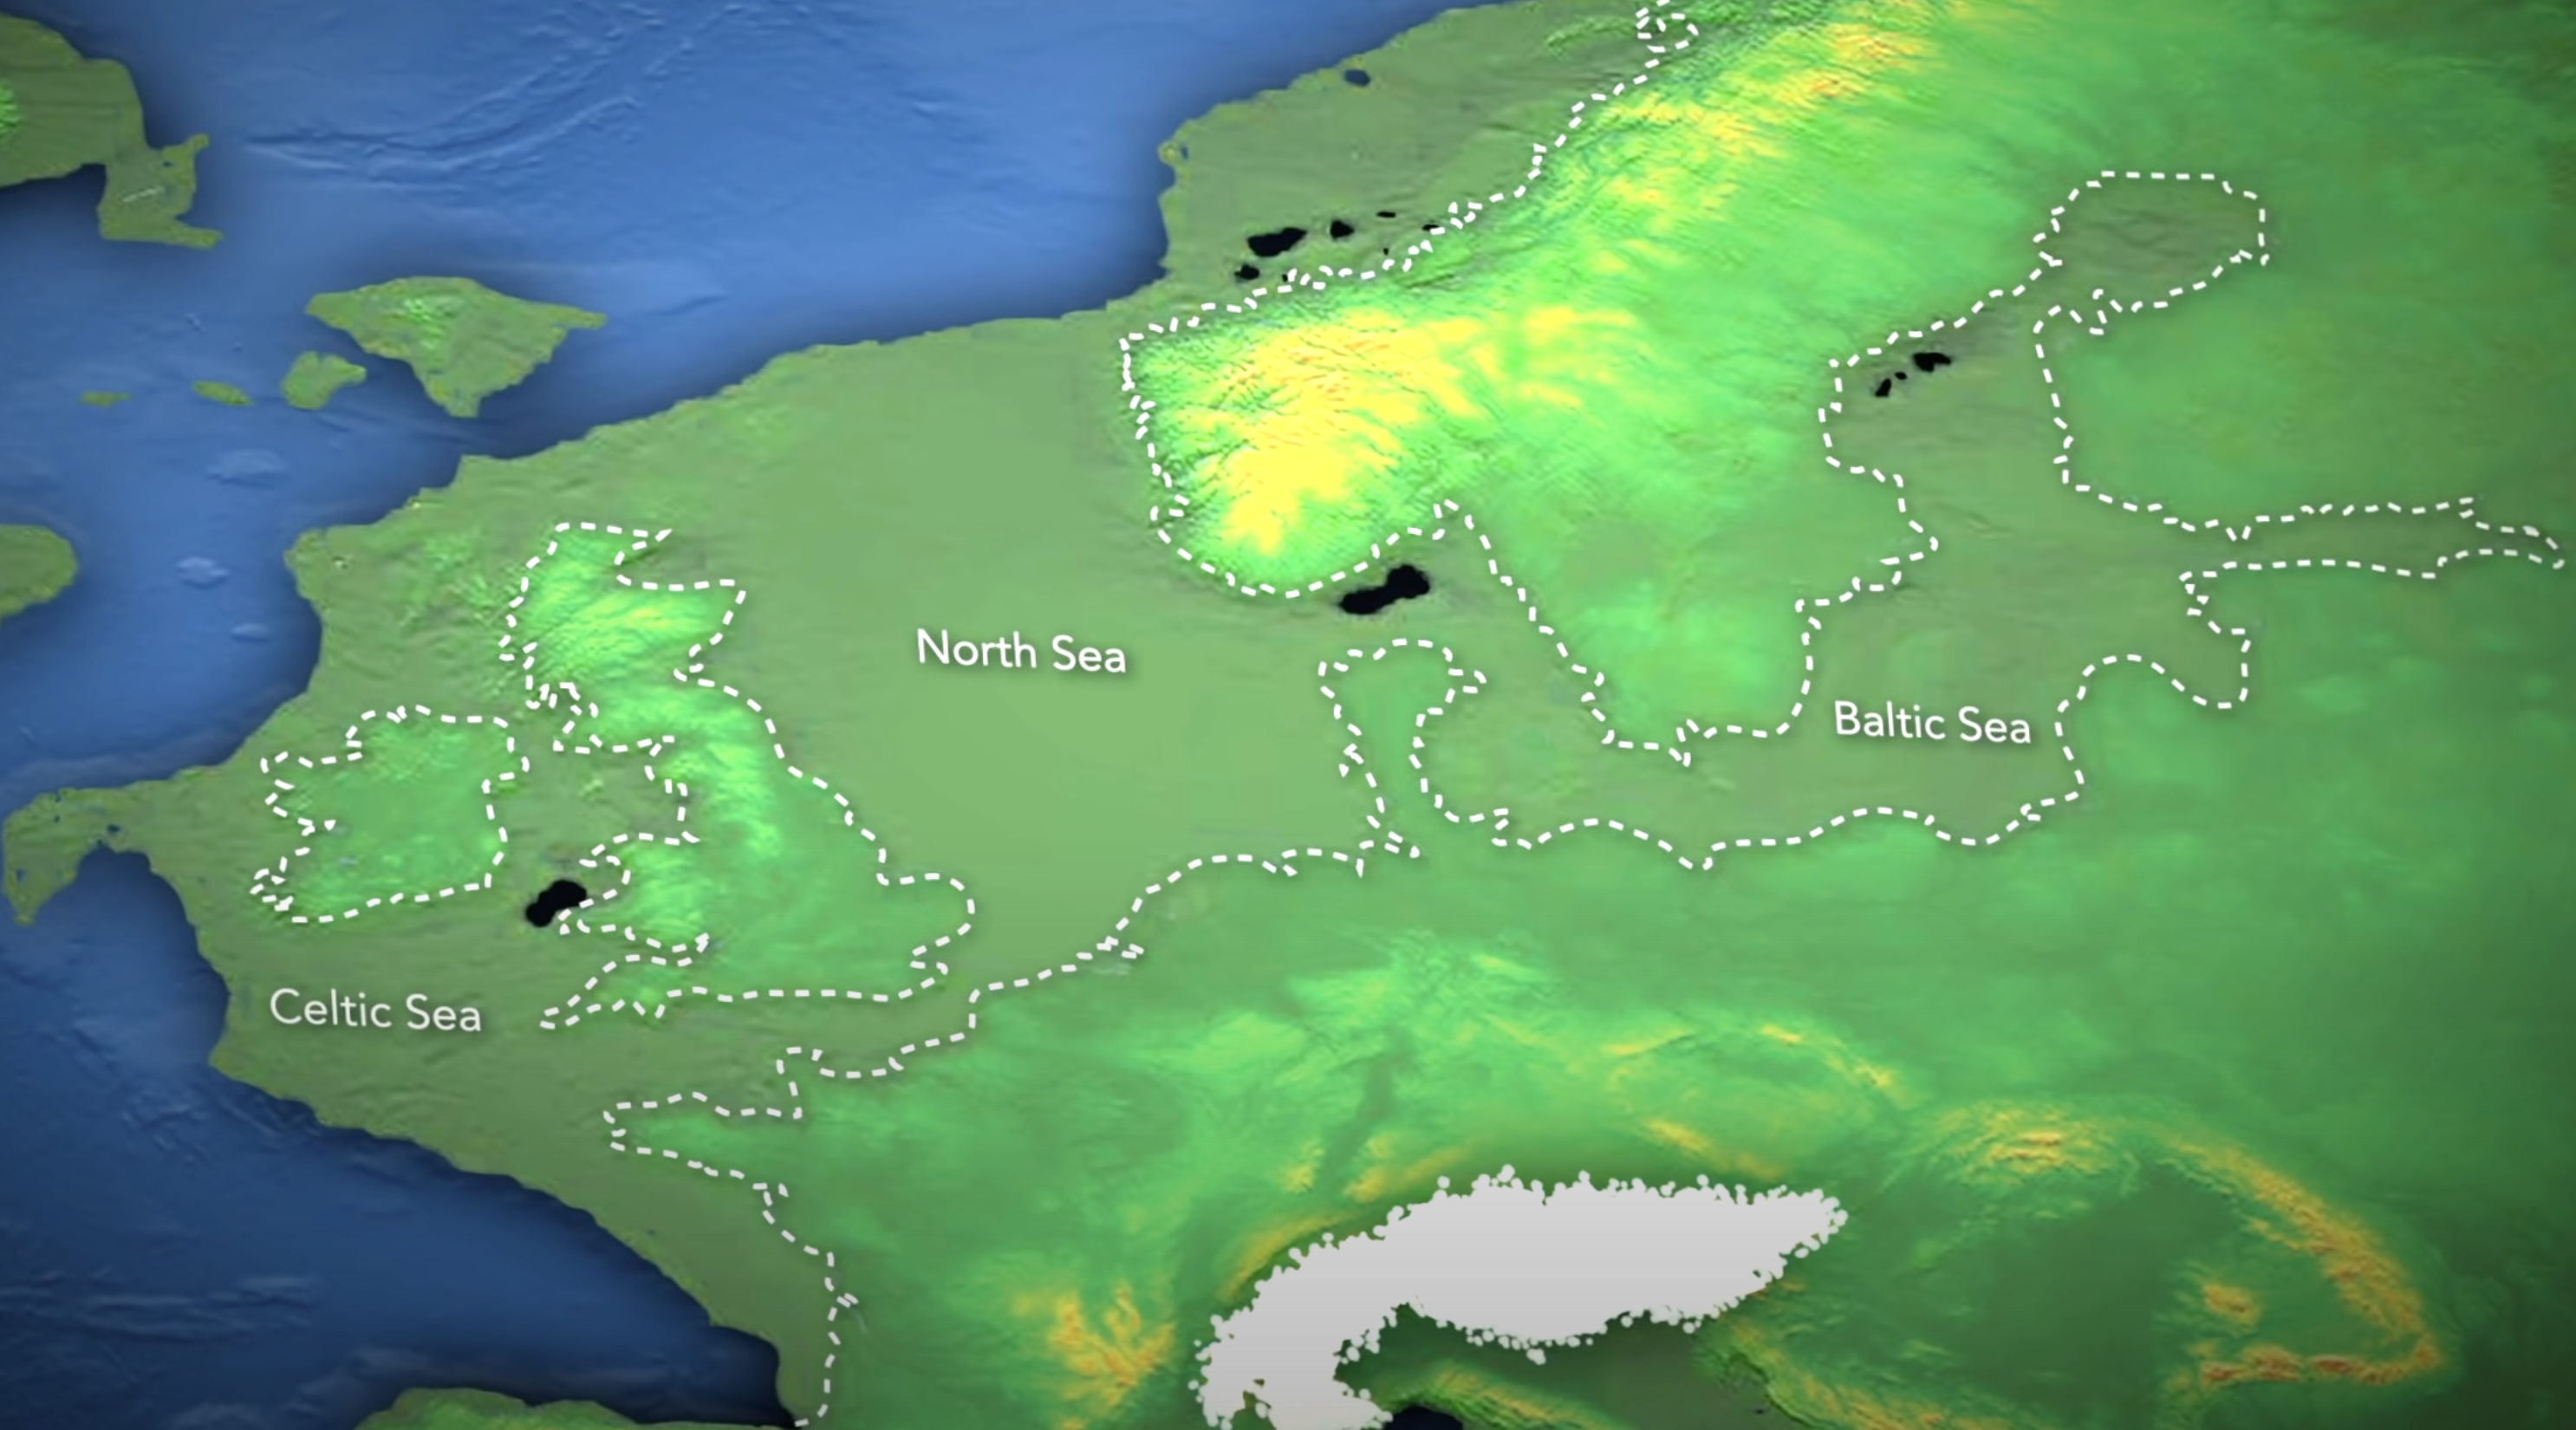
\includegraphics[width=0.65\textwidth]{land3.png}
\end{center}

This Ice Age also changed the biogeography of the connecting lands. One example from the Beringia land mass which brought forth the first humans to the other side of the world. There was also Animals that could freely move from Asia to the Sundaland. This was due to the land mass being exposed. Some of these animals were the Elephants, Rhinos, Apes, and Tigers. During the LGM the western United States had many basins that filled up to form large lakes. Some of these lakes were Lake Bonneville and Lake Lahontan. In Siberia, the Yensei and Ob Rivers were cut off from the Arctic Ocean due to the ice sheets, making them pool water and forming the west Siberian lakes. Back in the western United States, scientists found out that Lake Bonneville was filled in due to evidence of terrances formed by the lakes waves. There was also evidence in the form of signficant deltas that were formed at the mouths of major canyons.

\end{document}